\setchapterpreamble[u]{\margintoc}
\chapter{电路部署}
\labch{deploy}

\setlength\parindent{2em} 本章将进行电路的部署,即将继电器电路与生活用电器连接。本次选择了讲述方便、便于演示、功率小,安全性高的台灯最为演示用案例。最终将其部署成一个联网、智能化的台灯。

\section{电路规划}

\setlength\parindent{2em} 原台灯的电路简图如图\reffig{normallightori}所示。原台灯中已经有一个开关,位于火线上、镇流器之前,直接控制220V的通断。本次想要形成的效果是:两个开关分别独立,两个开关同时断开时,电路开路;否则电路为通路。换句话说,假设继电器与开关分别为A、B,则电路的通断状态R = A || B。

\begin{figure*}[h!]
	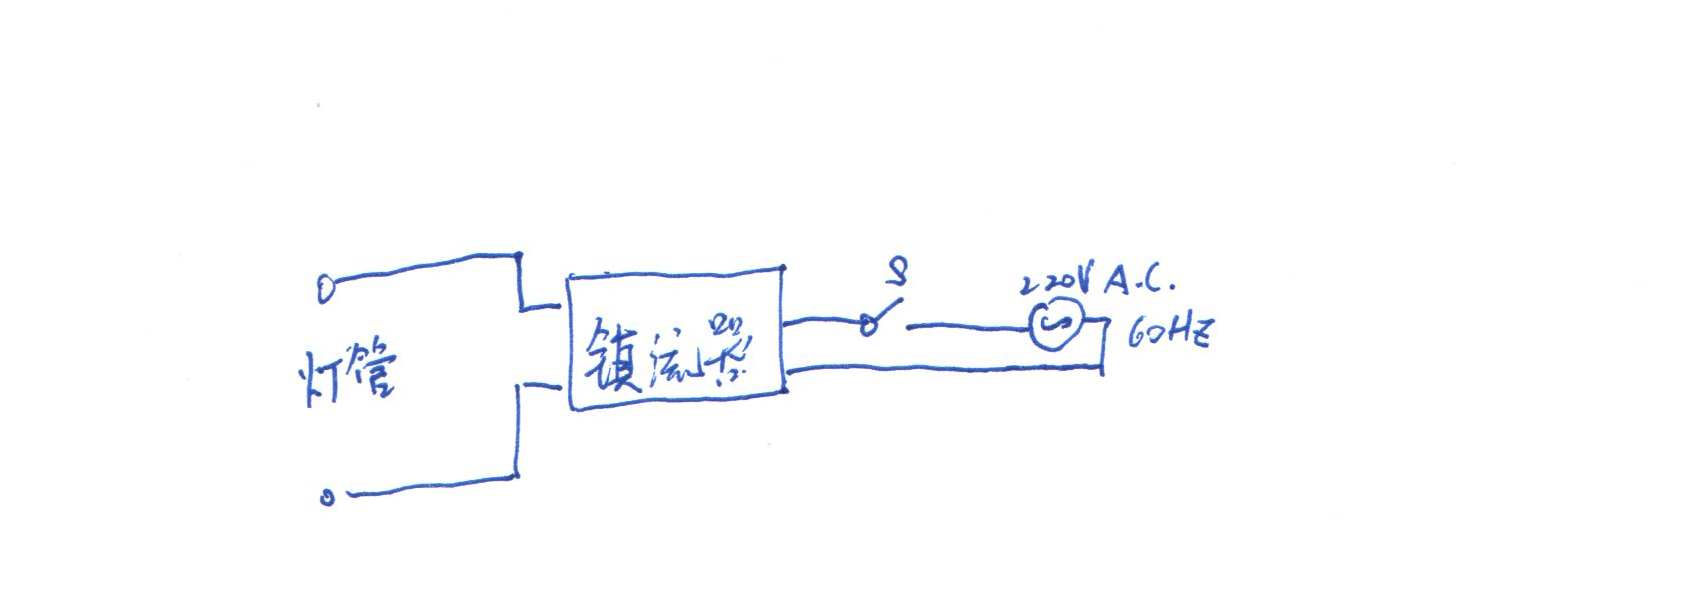
\includegraphics[width=\textwidth]{lightori}
	\caption[lightori]{原台灯的电路图}
	\labfig{normallightori}
\end{figure*}

\par 为实现此目的,需要将开关与继电器并联,最终形成的电路图如图\reffig{normallight}所示。继电器与开关并联,同时置于火线上。继电器的5V供电通过USB接口单独引出,利用220V AC-5V DC的降压模块供电。最终整个电路即可完成。

\begin{figure*}[h!]
	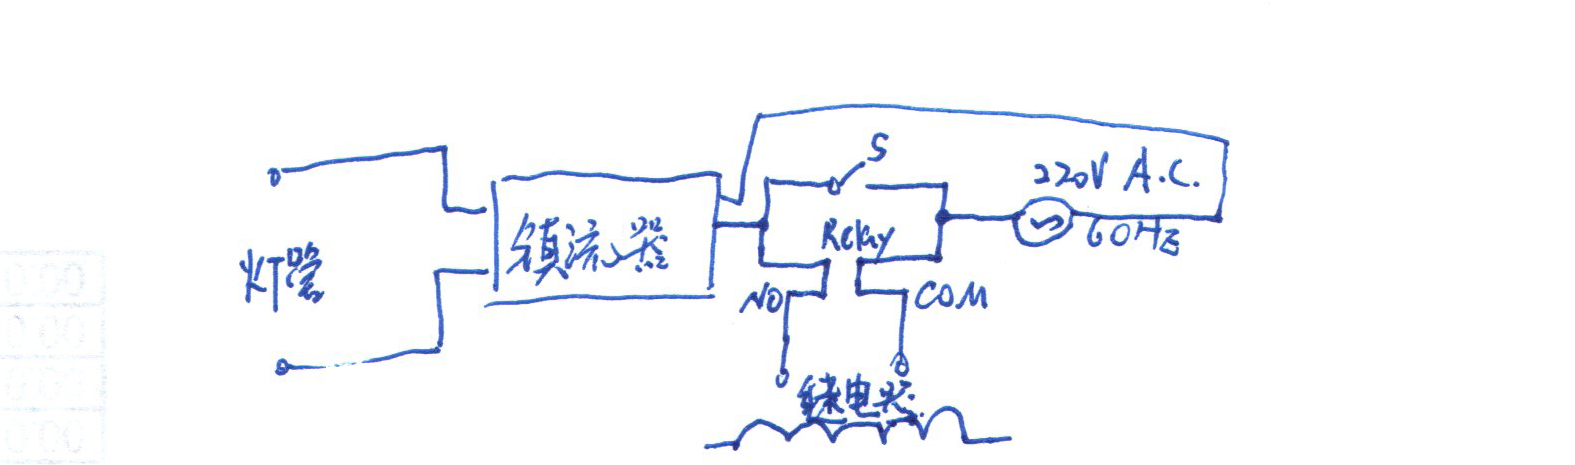
\includegraphics[width=\textwidth]{light}
	\caption[light]{部署后台灯的电路图}
	\labfig{normallight}
\end{figure*}

\section{成果展示}
\setlength\parindent{2em} 实验效果如下所示:

\begin{figure*}[h!]
	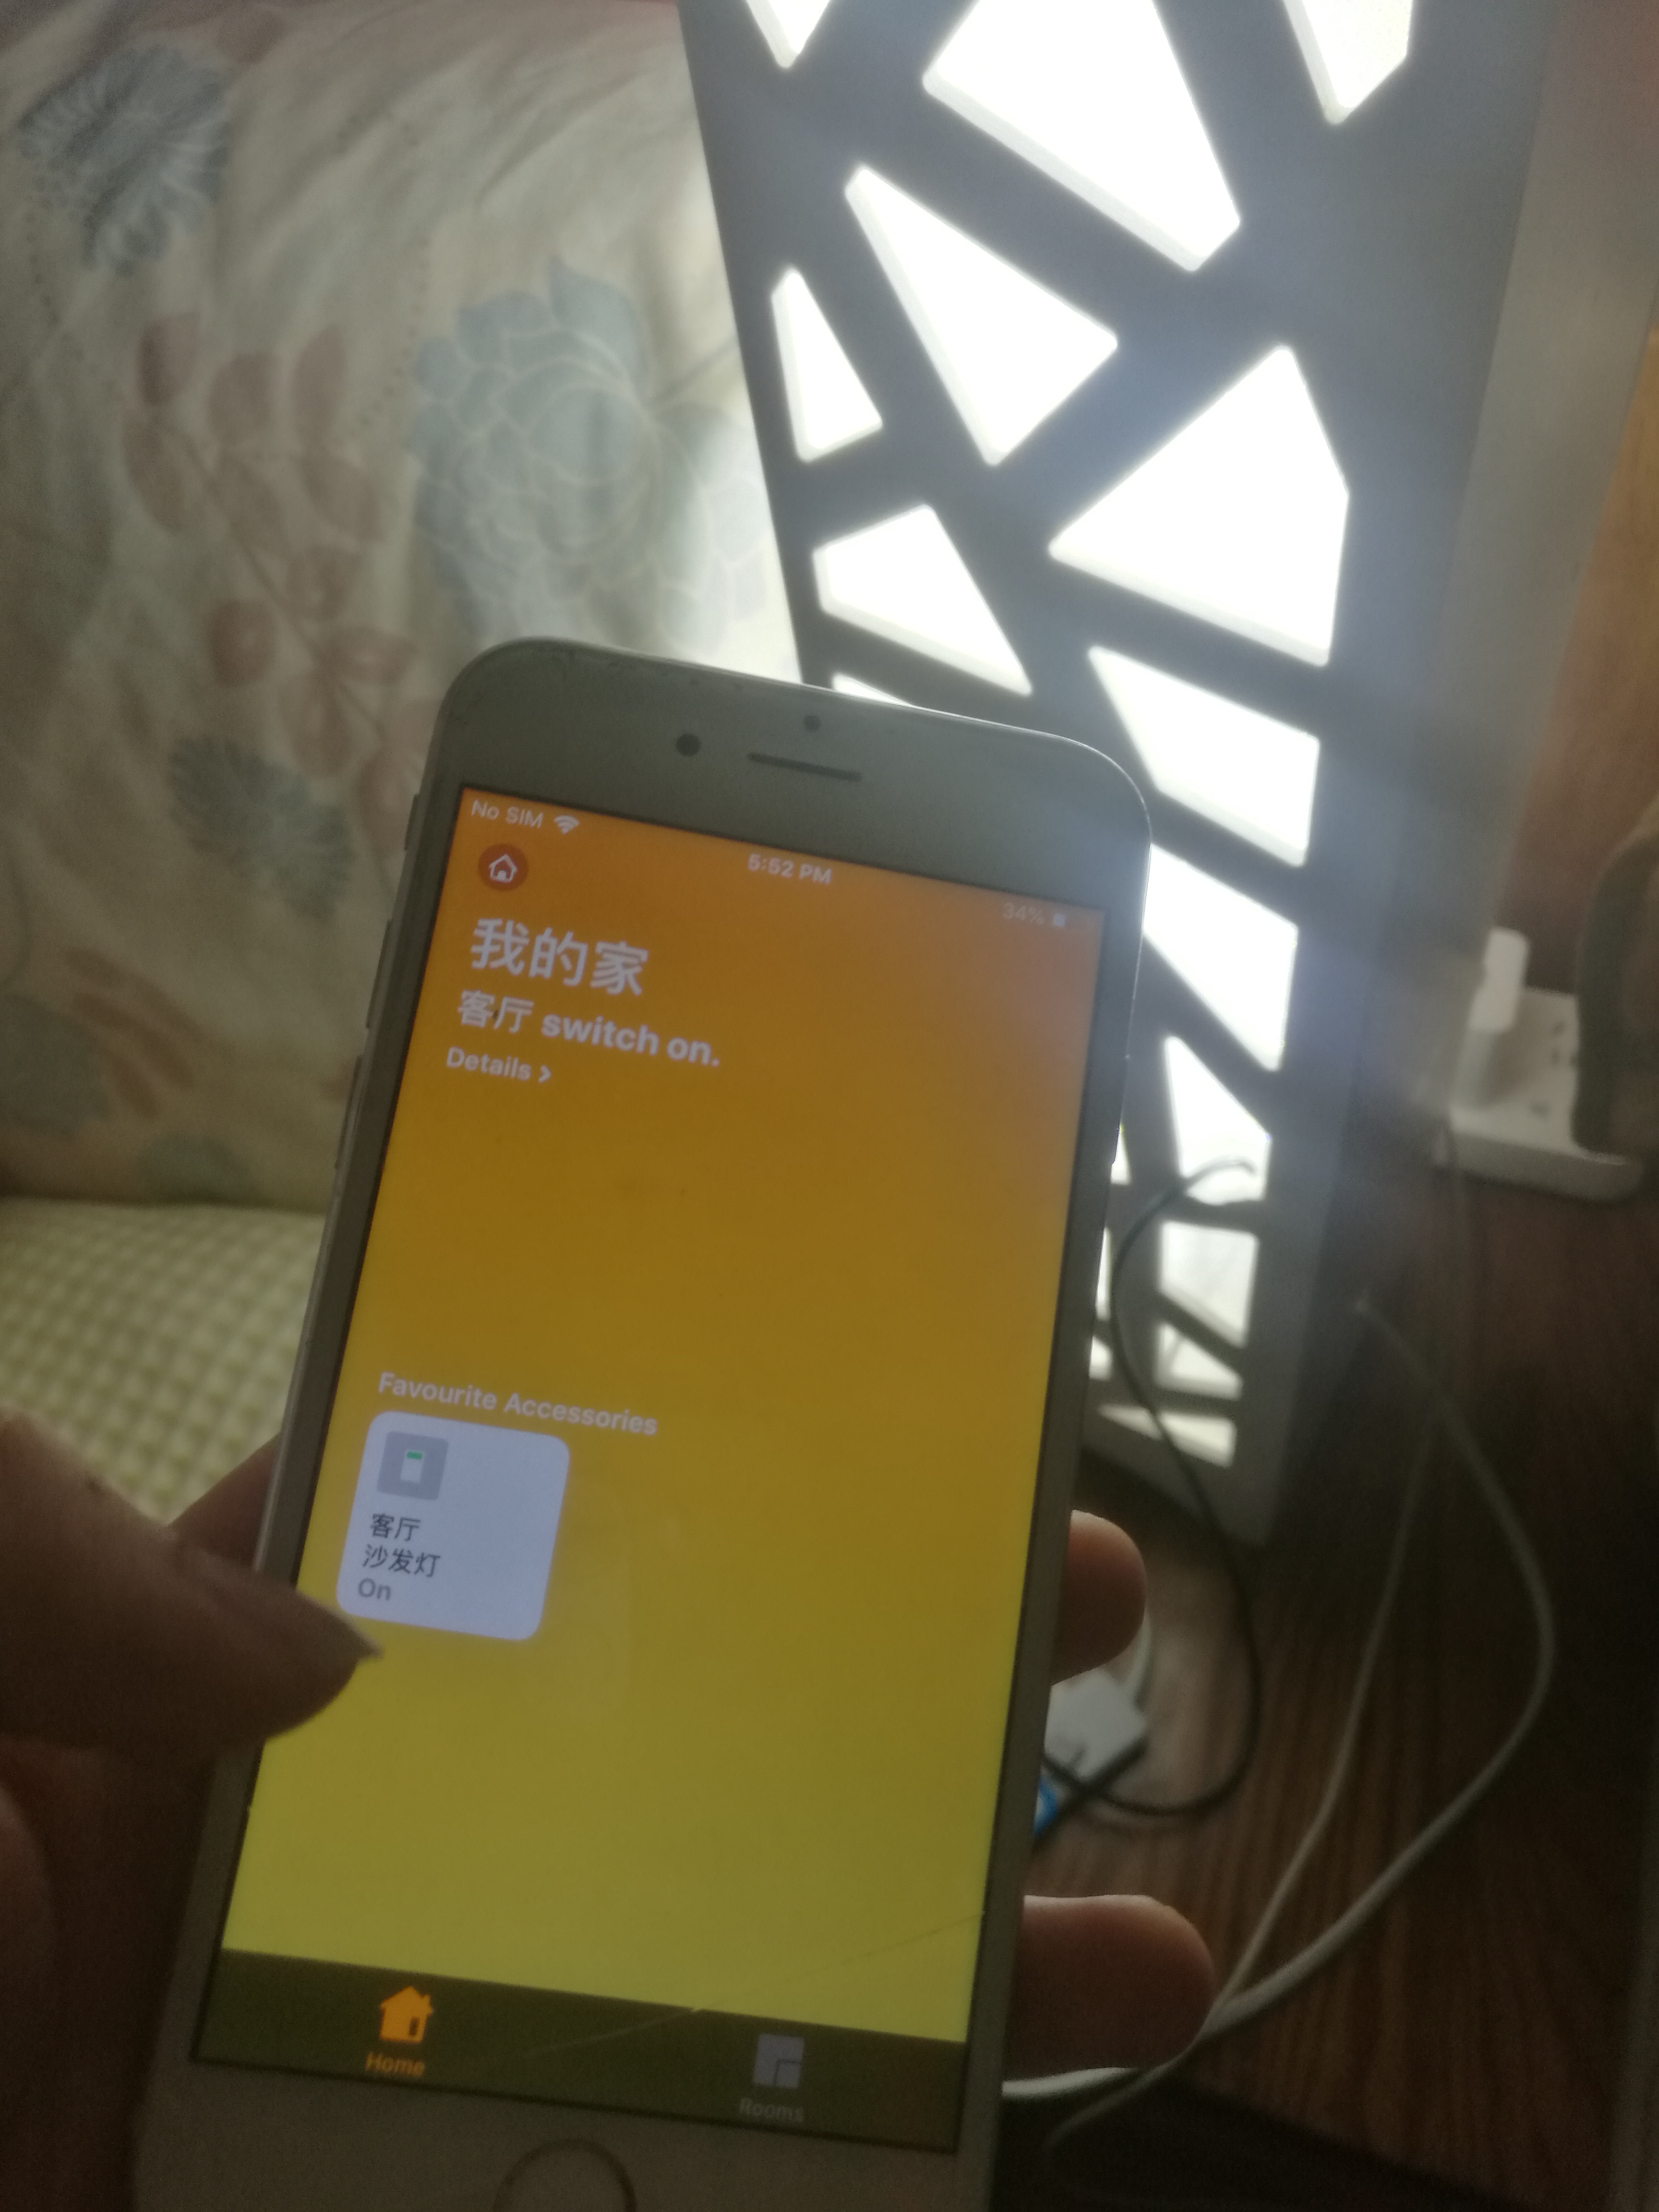
\includegraphics[width=\textwidth]{res}
	\caption[res]{效果图1}
\end{figure*}

\begin{figure*}[h!]
	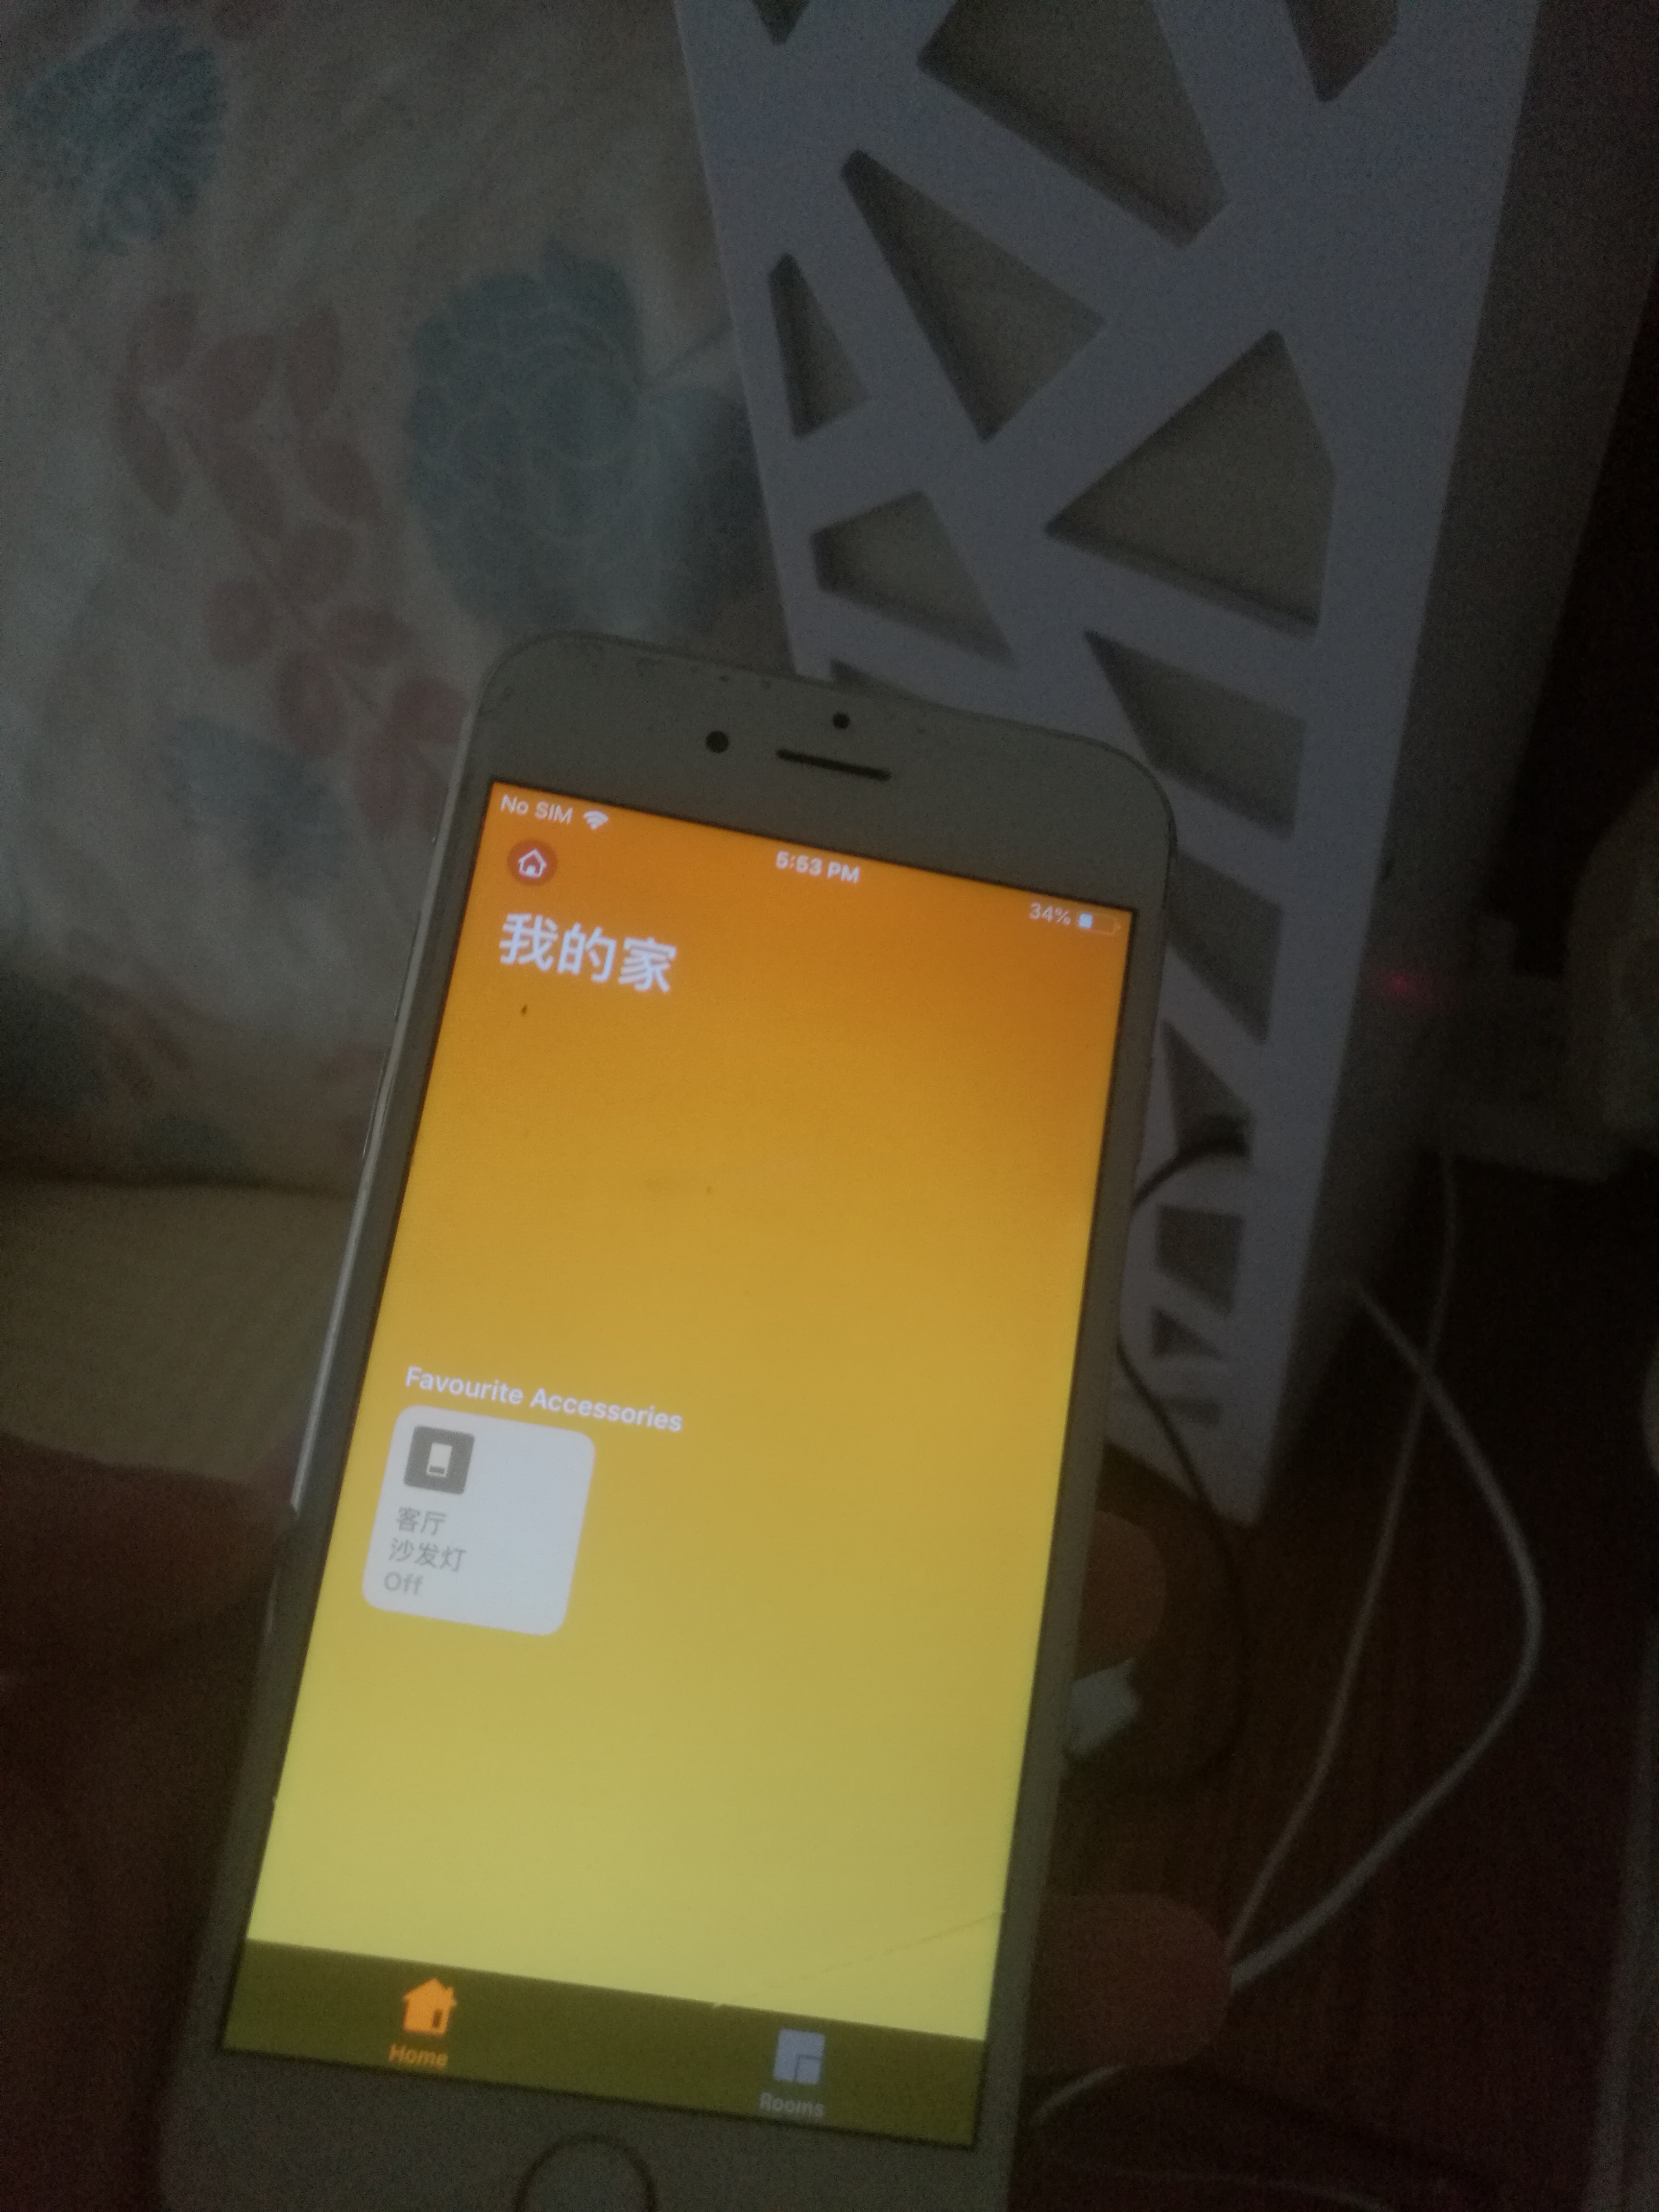
\includegraphics[width=\textwidth]{res1}
	\caption[res1]{效果图2}
\end{figure*}
